%Se puede anexar cualquier material que los alumnos estimen pertinente.

\subsection{Respuestas a las entrevistas}

\begin{itemize}
    \item Juan Alarcón Fuentes, Taller.
    \begin{enumerate}
        \item Tranquilidad, sentimiento de grupo, es grato.
        \item Lo entretenido del trabajo, que no es monótono. El logro es el
        perfeccionamiento de la técnica propia.
        \item Seguir aprendiendo, perfeccionarse.
        \item El deporte. Organizar más eventos deportivos. Más motivación por
        parte de los compañeros.
        \item Si, me gustaría tener más tiempo para poder realizar otras
        actividades.
        \item Establecerse más, tener un equipo conformado y estable.
        \item Las tallas.
        \item El 17 de Septiembre, porque se hacen asados y actividades fuera
        del trabajo.
        \item Más de uno. Compañeros de trabajo, desempeño laboral y como
        amigos.
        \item El Sábado, jugando en el club de tenis.
        \item Si me veo, con más experiencia. Podría comprar mis propias
        herramientas, pero no...
        \item Más de una persona. El equipo en general se lleva bien con
        todos.
        \item Si, porque considera que es una pega bonita. El hacer cosas
        propias es gratificante.
        \item El tratar de hacer las cosas que están a tu alcance y que te
        hagan feliz.
        \item El deporte o el baile, la música.
    \end{enumerate}
    \item  Paola, Taller.
    \begin{enumerate}
        \item Me agrada.
        \item Mi trabajo, la confianza. Todo con la mejor dedicación.
        \item "Ganar plata" jaja. Es gratificante, me gusta el trabajo.
        \item El compañerismo. Compartir más con la gente. Más preocupación.
        \item Si, con respecto a como llevar el taller, la organización del
        mismo.
        \item "Que el jefe tenga más plata", el cumplimiento de los plazos en
        el trabajo.
        \item ... la solidaridad de algunos.
        \item Antiguamente, eran los paseos de viernes-sábado a unas cabañas.
        \item "Yo". Considero que hago bien mi trabajo, muy preocupada de los
        detalles.
        \item El viernes en la tardecita, cuando me voy, tenemos una cena con
        mi familia.
        \item Si, dependo de este trabajo.
        \item De un compañero que todavía está acá, que me ayudó a pedir el
        crédito para mi casa.
        \item Sí, porque no había otro taller de joyería!.
        \item La disposición mía a hacer cosas que los demás no quieren hacer,
        y mi capacidad para ser directa y precisa.
        \item Una vez a la semana recibir un tipo de majases o charlas con
        otros temas fuera del tema de trabajo  (libros, películas, etc.).
        Un "break" para hacer cosas, como tomar café.
    \end{enumerate}
    \item Miguel, Taller.
    \begin{enumerate}
        \item Algo bueno, que me ha dado un mejor pasar en la vida.
        \item El llegar a ser joyero. Descubrir que uno tiene talento.
        \item El bien de mi familia.
        \item Me llevo bien con todos. Hay cosas que me gustaría más, el
        deporte, por lo social.
        \item Claro, pero si digo que sí, voy a "dar jugo", no me pagarán más
        por ello.
        \item Acá los motiva el jefe. Se preocupan por el lado familiar, super
        bien.
        \item Bien, el grupo de trabajo tiene buena relación. 
        \item Los aguinaldos, me gusta andar en mi trabajo.
        \item Un compañero que se fue. Los demás bien, normales como uno.
        \item El jefe.
        \item El fin de semana. El día Viernes porque tengo competencias
        deportivas.
        \item El jefe, don Iván.
        \item Volvería a las Fuerzas Armadas, pero después igual trabajaría en
        la Joyería, pensando más.
        \item Pensando en la muerte:"No quiero que me recuerden, quiero estar con mi gente no más
        cuando me muera". En la joyería, le gustaría que le recuerden la
        amistad.
        \item Deporte! Que hagan más deporte.
    \end{enumerate}
    \item Anónimo, Taller.
    \begin{enumerate}
        \item Agradable, sí, me gusta lo que hago.
        \item "Le caigo mal a todos así que..." peleador de las causas
        perdidas. Defender a mis compañeros y mis cosas. Algunas veces, el
        trabajo.
        \item "El sueldo a fin de mes".  Es  que yo se que en un par de tiempo
        más voy a tener que ser independiente, y trabajar más para mí.
        \item Más organizaciones sociales y eventos. Como el paseo de fin de
        año.
        \item Sí, me gustaría aprender más de mis compañeros de trabajo.
        \item La expansión que ha tenido, gracias al orden y perseverancia.
        \item Son unidos, lo normal.
        \item Mi trabajo en sí, siempre hay cosas distintas, es bueno.
        \item El jefe, la lleva.
        \item El Viernes, porque es el último día de la semana, porque tienes
        libertad de hacer lo que quieras.
        \item Ya independiente, a menos de ser gerente general jaja.
        \item De mi Jefe.
        \item Si, de hecho.
        \item Que cantaba bien, porque paso cantando. Que soy una persona
        alegre.
        \item Un vez al mes juntarnos e ir todos a un partido o algo, para
        compartir ideas entre los demás.
    \end{enumerate}
    \item Gastón, Taller.
    \begin{enumerate}
        \item Una fuente de ingreso que cumple reglas, que en otros lados no
        se dan.
        \item Con conocimientos para mis compañeros y pegas que quedan buenas.
        \item La fuente laboral, me gusta lo que hago, pero mi meta es la
        estabilidad.
        \item Paseos, volver a hacer los paseos a fin de año.
        \item Si, de todas maneras. Acá estas limitado al catálogo, no creas
        cosas nuevas.
        \item Un reconocimiento en el mercado y estabilidad laboral.
        \item Igual hay una preocupación por parte de los demás.
        \item Que el jefe "se rajó" con una pantalla gigante y con un asado.
        \item Si, hay un cabro que es bien sociable, siempre está en todas las
        actividades, etc.
        \item El Viernes, porque se acaba la semana, el fútbol.
        \item No me lo he planteado. No me hago planes a largo plazo. Veo
        estar aquí como una transición.
        \item Del jefe que todavía nos mantiene aquí.
        \item Si, porque ha sido bien interesante para mi trabajar aquí. He
        aprendido harto aquí.
        \item Mi trabajo. Yo igual se harto, y cacho más que la mayoría. Que se
        acuerden que era buena onda con los demás.
        \item Más actividades que levarán a tener mejores relaciones entre
        todos fuera del trabajo.
    \end{enumerate}
    \item Ricardo Pedraza, Taller.
    \begin{enumerate}
        \item Estoy acá porque no hay nada mejor.
        \item Que tengo la mitad de un taller acá. Amigos no, tengo
        compañeros.
        \item Quiera independizarme y tener un taller. Porque no hay horario
        de salida, si sales antes se enojan.
        \item Acá cada uno mata su chancho.
        \item No hay incentivos por ser creativo. Yo sólo por
        fuera, sí.
        \item Que se mantiene estable.
        \item "Yo no más poh". Difícil.
        \item Que celebran los cumpleaños cuando el jefe dice. El
        hombre es un dictador. Se fueron los otros.
        \item Una compañera que s preocupa. Gladys.
        \item Los Sábados y Domingo, porque estoy con mi familia, 4 hijos (y
        pronto 5).
        \item Cómo independiente.
        \item De la Gladys. A estado siempre.
        \item No, no volvería. Por los tratos.
        \item Que era trabajador, rápido.
        \item Incentivos monetarios, más motivación. No hay paseo, no hay
        nada. Aumento de sueldo.
    \end{enumerate}
    \item Alarcón Reyes, Taller.
    \begin{enumerate}
        \item Si, por supuesto que si me gusta. Antes trabajaba en un lugar
        donde cada uno era su jefe. Me costó un poco acostumbrarme, pero no he
        tenido ningún problema.
        \item ... Uno el trabajo lo hace bien, y eso es reconocido.
        \item No tiene mucho sentido el pensar en otros puestos del trabajo.
        \item La parte social. Que cada cierto tiempo haya un encuentro con la
        familia, todo eso.
        \item Si, tratar de aprender otro tipo de trabajo, pero acá los
        puestos ya están limitados a un puesto de trabajo.
        \item Que ha cumplido todas las cosas de la ley. Encuentro que la
        empresa es muy buena en lo social.
        \item La relación entre los compañeros de trabajo, el respeto entre
        los compañeros.
        \item Una celebración del 18 en la casa del jefe, con nuestros
        familiares.
        \item El Jefe, Paola Miranda, Gladys Reyes.
        \item El día Viernes. La jornada acá es muy larga, son más horas de lo
        que realmente deberían ser.
        \item "Ya no me veo jajajaj". Aprendiendo otras cosas. 
        \item El jefe que me dio pega.
        \item Si, por supuesto. Porque había otro sobrino que ya estaba
        trabajando acá, y ya conocía como era acá el trabajo.
        \item El respecto y la amistad a la gente.
        \item Falta algo como una charla educativa, temas de actualidad,
        charlas varias, temas fuera de la empresa. Eventos donde estemos todos
        juntos. No hay tiempo para conversar temas con los demás.
    \end{enumerate}
    \item Anónima, Vendedora.
    \begin{enumerate}
		\item Me siento bien, me gusta.
		\item Le ha enseñado a hacer otras cosas.
		\item Meramente compromiso, por dinero.
		\item Nada.
		\item La uso!, decorando el local.
		\item El aumento de la cantidad de trabajo. 
		\item La afinidad entre los compañeros.
		\item La celebración de los cumpleaños, cosas que se han mantenido.
		\item El jefe.
		\item El viernes, ya que termina la semana.
		\item No sé, tengo un futuro incierto.
		\item EL jefe, cuando se le pilla en buena, es buena gente.
		\item No, el horario es aburrido, el rubro también.
		\item Como la graciosa y creativa.
		\item Una travesura al jefe entre todos o salir del lugar del trabajo.
    \end{enumerate}
    \item Maribel, Secretaria.
    \begin{enumerate}
		\item Por trabajo solamente.
		\item Estoy restringida al cargo solamente. Responsabilidad.
		\item Mi hijo.
		\item La comunicación entre compañeros.
		\item Si, pero estoy acotada al cargo solamente.
		\item El crecimiento de la empresa, más clientes.
		\item Son buenas personas.
		\item Fiestas y celebraciones de navidad.
		\item La Paola, es como la mamá de todos.
		\item Viernes, termina la semana y comparto con mi hijo.
		\item No me veo.
		\item Una compañera, desde el día en que llegué, me ha ayudado en todo.
		\item No, he estado 10 años y sigo igual.
		\item La creativa, la que adorna el local.
		\item Hay mucha disconformidad, se podría hacer un grupo y discutir sobre ello.
    \end{enumerate}
    \item Vendedora Anónima 1, Sucursal 
    \begin{enumerate}
        \item Opción Laboral .
        \item No lo sabe, lo desconoce.
        \item Sueldos.
        \item Distribuir mejor los deberes, definir mejor los cargos.
        \item Si, en ventas no hay mucho pero se pueden varias mucho haciendo ofertas, promociones. Acá vendemos oro y plata, entonces la gente que viene tiene el dinero para comprarlo, por lo que no se hacen muchas ofertas.
        \item Prestigio de la joyería, es un trabajo garantizado, con respaldo.
        \item Ambiente , somos 2 vendedoras, nos entendemos y el horario nos favorece, nos complementamos, todo bien.
        \item No participo, no me gusta mucho.
        \item El Jefe es fundamental, el hace que todo funcione, si el no está no funciona el negocio.
        \item El viernes, por el fin de semana.
        \item No se puede proyectar, tengo planes para migrar.
        \item El Jefe y su compañera ha sido un aporte.
        \item No lo aceptaría, no estoy 100\% complacida.
        \item Como sincera, transparente, directa.
        \item Un cara a cara para sanar cosas y unirse mas. Reuniones al mes con el Jefe presente.
    \end{enumerate}
    \item Vendedora Anónima 2, Sucursal 
    \begin{enumerate}
        \item Cómoda porque no hay presión.
        \item Buen contacto con los clientes, porque se es simpática.
        \item Por mi hija, hay que mantener la casa.
        \item Juntarse fuera del trabajo, cumpleaños, etc, es muy entretenido.
        \item Lo que mas hago es ser creativa, aunque prefiero trabajar en taller no en ventas.
        \item Crecimiento de la empresa, el avance tecnológico para registrar todo en el computador.
        \item Comparto con todos y todos tienen características especiales, todos son preocupados.
        \item Festividades, como esperar el partido de Chile para el mundial en el taller.
        \item El Jefe, el maneja todo bien, las vendedoras tienen respeto del jefe porque nos escucha.
        \item Todos, aunque el Sábado y Domingo, para estar con mi hija y me extraña mucho (tiene 4 años).
        \item Me veo en el taller, en lo que más me gusta.
        \item El Jefe, no por patera, nos ayuda mucho y mi compañera también.
        \item Si, ha sido el mejor lugar donde he trabajado, incluso me despidieron y volví a pedir el trabajo y me aceptaron, tienen todo al día.
        \item Disposición, responsabilidad y alegría!
        \item Hacer reuniones una vez al mes para discutir de todo y llegar a acuerdos.
    \end{enumerate}
\end{itemize}


\subsection{Imágenes}

    \begin{figure}[h!]
    \centering
        
\includegraphics[height=7cm]{img/sucursal.jpg}
        \caption{Sucursal.}
    \end{figure} 
    \begin{figure}[h!]
    \centering
        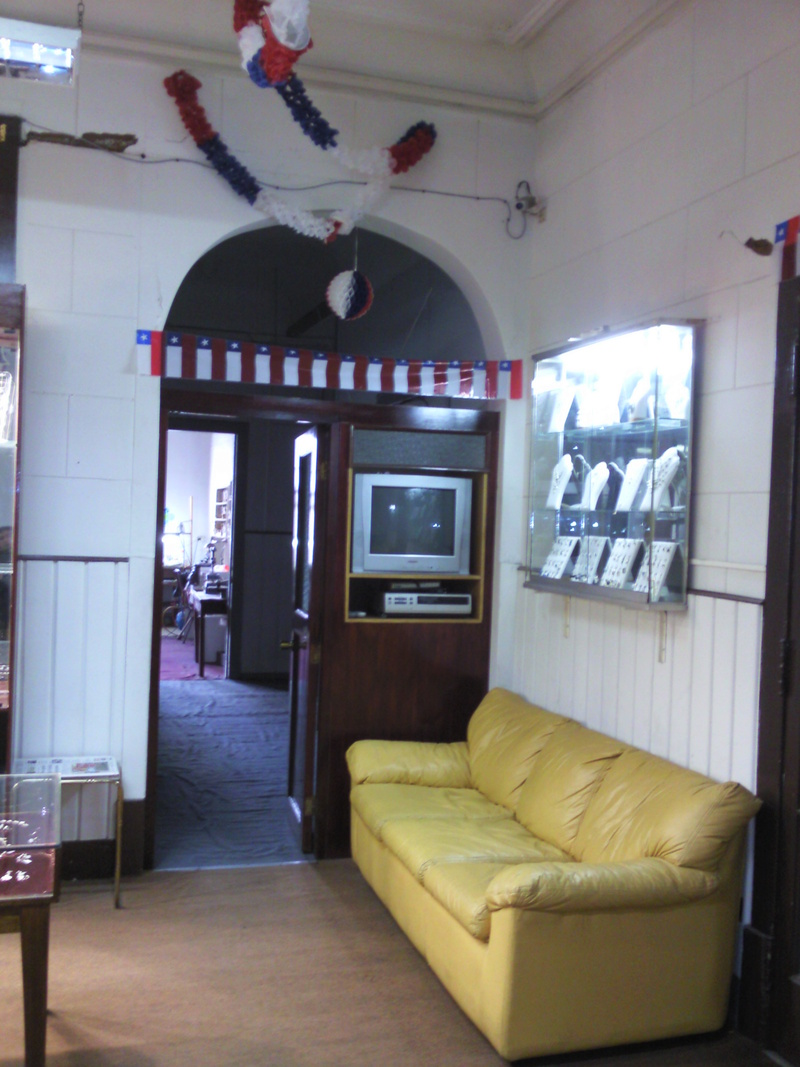
\includegraphics[height=7cm]{img/central1.jpg}
        \caption{Sede Central.}
    \end{figure}
    \begin{figure}[h!]
    \centering
        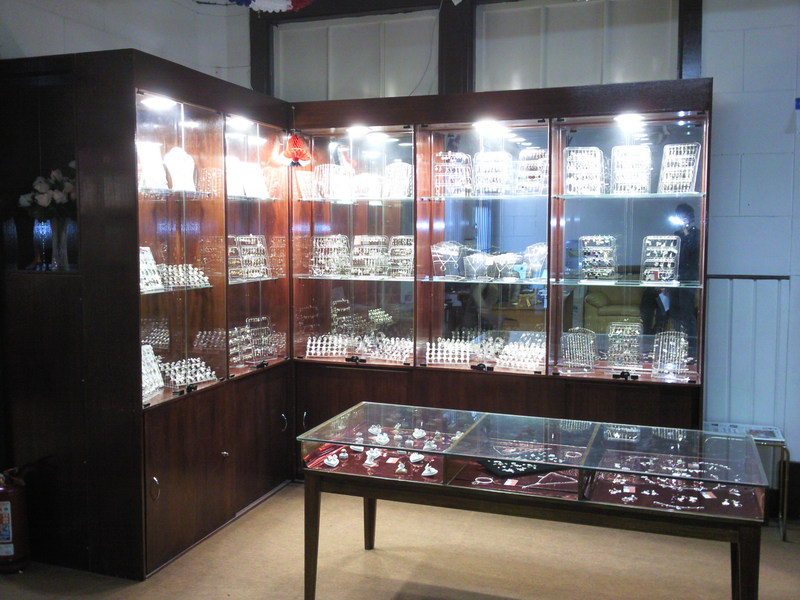
\includegraphics[height=6cm]{img/central2.jpg}
        \caption{Sede Central.} 
    \end{figure} 
    \begin{figure}[h!]
    \centering
        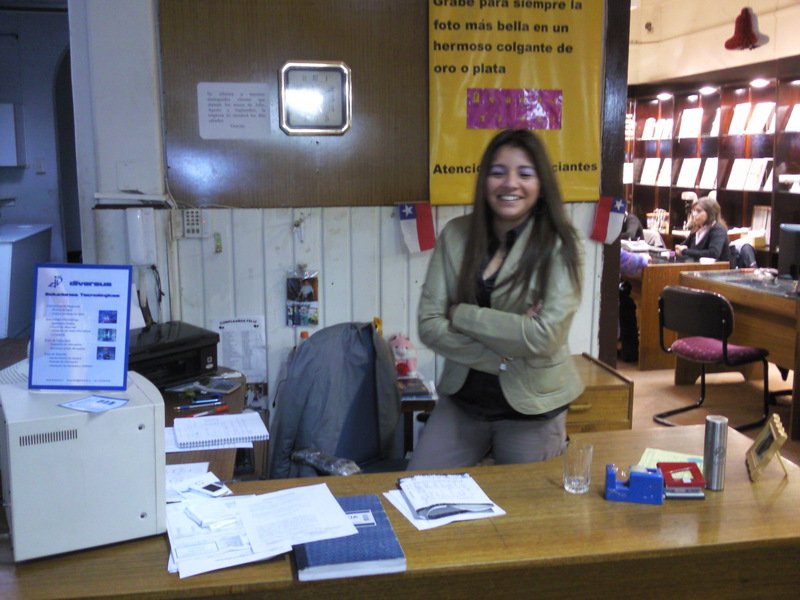
\includegraphics[height=6cm]{img/secretaria.jpg}
        \caption{Secretaria en Entrevista.}
    \end{figure}
